\documentclass[../Thesis.tex]{subfiles}
 
\begin{document}
 
\section {Signal Processing}
\subsection {Short-Time Fourier Transform}
The Short-Time Fourier Transform is the most used method of time-frequency analysis. The main concept relies on multiplying $x(t)$ with an analysis window $y*(t-r)$ and then compute the Fourier Transform of this windowed signal.

\begin{figure}[h]
\centering
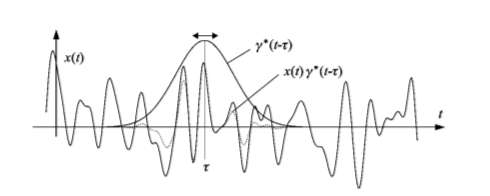
\includegraphics[width=0.5\textwidth]{stft.png}
\end{figure}
 
STFT formula:
\[ F_x^\gamma (\tau, \omega) 
= \int_{-\infty}^{\infty} x(t) \gamma *(t - \tau) e_{}^{-j \omega t} \mathit{d} t .\]
 
In a digital environment we will use the discrete formula instead:
\[ F_x^\gamma (\mathit{m}, e_{}^{j \omega}) 
= \sum_{n} x(n) \gamma *(\mathit{n} - \mathit{mN} e_{}^{-j \omega \mathit{n}}) .\]
 
The window $y*(t-r)$ suppresses $x(t)$ outside a certain region and the FT outputs a local spectrum.
The FT is complex valued, so we use a spectrogram to display it. This also helps us for further processing the signal. In our application we will use the amplitude spectrum as input for our neural network. The spectrogram is created by computing the squared magnitude of the STFT:

\[ {\mathit{S}_x (\tau, \omega)} 
= |F_x^\gamma(\tau, \omega)|_{}^2
= |\int_{-\infty}^{\infty}x(t) \gamma * (t - \tau) e_{}^{-j \omega t} \mathit{d} t|_{}^2 .\]
 
After we are done filtering the spectrum, we will need to reconstruct the signal to get an audio back. A reconstruction of x(t) is possible and is done so easily by the Inverse Short-Time Fourier Transform (ISTFT) formula:

\[ x(t) 
= \frac{1}{2\pi}\int_{-\infty}^{\infty} \int_{-\infty}^{\infty} F_x^\gamma(\tau, \omega) g(t - \tau)e_{}^{j\omega t} {\mathit{d} \tau} {\mathit{d} \omega} .\]
 
We will implement the equivalent discrete formula to reconstruct our signal. 
\subsection {Spectrogram}

A spectrogram is the visual representation of the frequency spectrum for a given signal. Spectrograms show energy or dB (by color) as a function of time and frequency. To form a spectrogram the sampled data must be broken into overlapping chunks and transformed by the Fourier transform into the magnitude of the frequency spectrum. Each chunk is then arranged one after another to better see the evolution in time of the signal. This process can be replaced by computing the squared magnitude of the STFT.

\begin{figure}[h]
\centering
\label {fig: spectrogram}
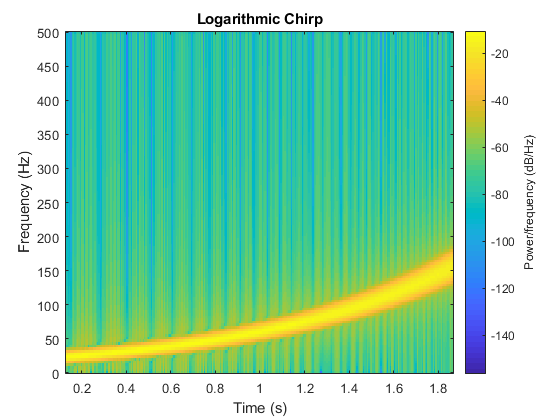
\includegraphics[width=0.5\textwidth]{spectro2.png}
\caption[width=0.5\textwidth]{Spectrogram}
\end{figure}

Working with frequencies proves to be easier than working with the waveform directly. A spectrogram can be edited and turned back into the corresponding waveform by a reverse process using ISTFT. 


\section {Deep Learning}
\subsection {Generalization}

In the early days of AI, the field solved mostly problems that are difficult for humans but relatively easy for computers, problems that can be described easily using mathematical rules. However, problems that we solve intuitively, such as recognizing objects or spoken words, were the real challenge of AI.

Deep learning is an answer to problems such as these, by making the computer learn from experience and creating a hierarchy of concepts in increasing difficulty of understanding. To understand a concept, the computer must understand a lot of simpler concepts first. The number of layers create a “deep” graph, hence one of the reasons for the name. Deep learning can scan large data sets and discover intricate structures by using the backpropagation algorithm. This method uses a so called “Artificial Neural Network” about which we will talk below. Mostly used is the convolutional neural network architecture. It is best known for the results in computer vision. Although convolutional neural network can be used to solve our problem, we chose the more suitable recurrent neural network as the architecture for our deep learning algorithm, seeing as our data can be viewed as sequential.

Deep learning greatly improved the state-of-the-art in object detection and speech processing. Deep recurrent networks brought breakthroughs in processing sequential data, while deep convolutional networks greatly improved the processing of images, video and even audio.


\subsection {Supervised Learning}

Supervised learning is the most common form of machine learning. The goal of supervised learning is to find a mapping from $x$ to $y$, given a set of pairs $(xi, yi)$ named training set. Here, $x$ will be the input(example) and $y$ the output (label or target).  Next, we will consider a simple problem that will help understand supervised learning better. Imagine we want to classify images based on what object they contain: a car, a dog or a house. A training data consisting of pairs of pictures and the correct label must be given to our supervised learning algorithm. Given a picture as input, the machine will give output a vector of scores, corresponding to the probability of the image belonging to each category. Because we actually know the correct answer, we can check how good the algorithm is by computing the error or “loss”. This measures how far the algorithm was from the right answer (label). The machine modifies some internal adjustable parameters to reduce this error. This is often referred to as backpropagation and the adjustable parameters as weights.
Stochastic gradient descent is the most common procedure for minimizing the loss. For a few inputs, the weights and the error are computed, along with the average gradient. The weights are adjusted according to this average gradient. The process is repeated multiple times for many small sets until a minimum average loss is obtained. This method can lead to finding a local minimum loss and staying there, without ever reaching the global minimum we desire.

\begin{figure}[h]
\centering
\label {fig: sgd}
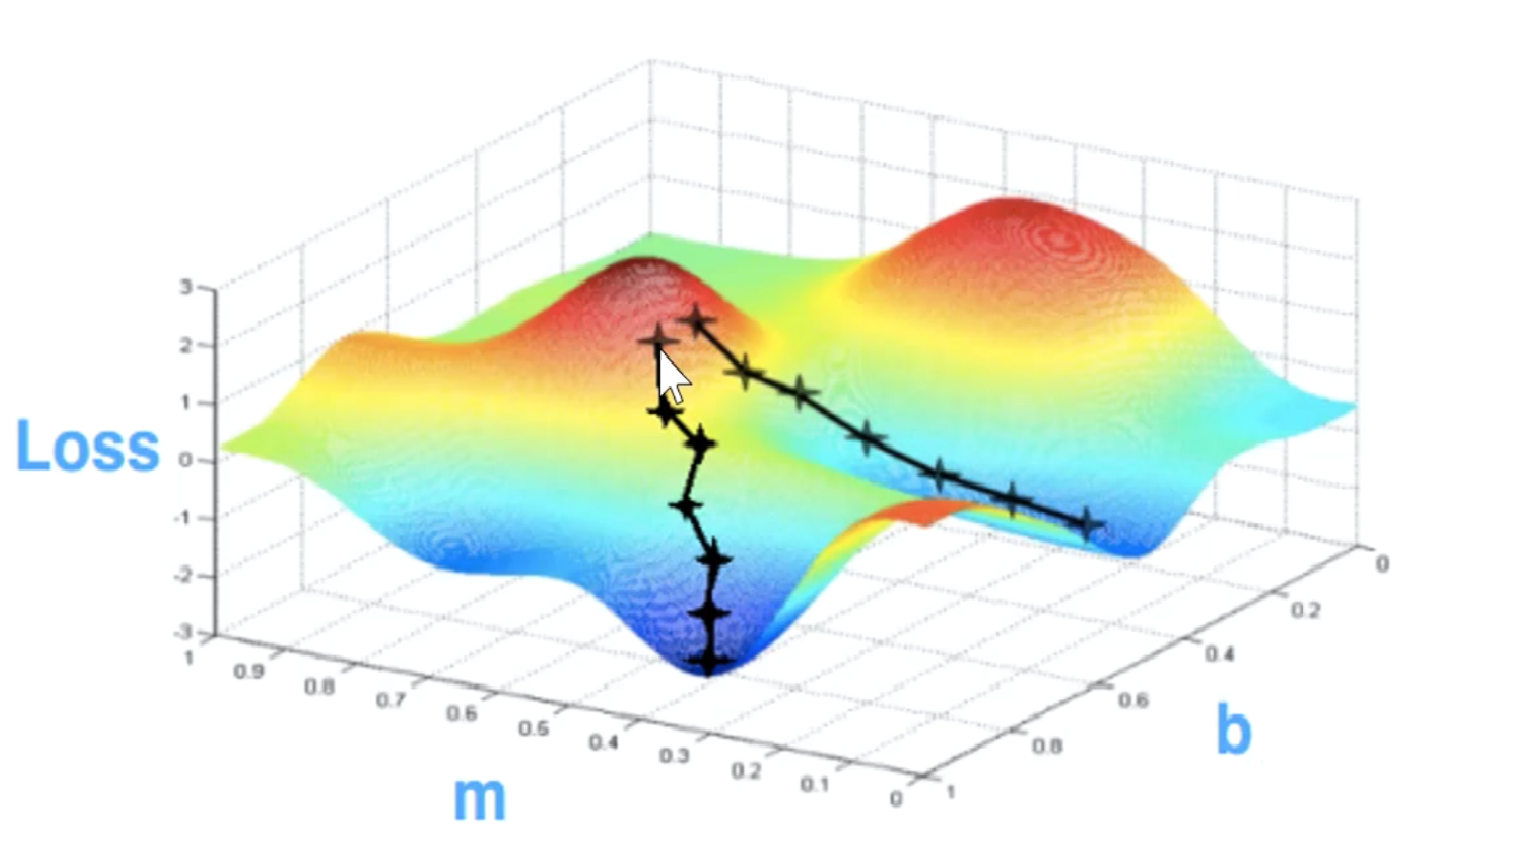
\includegraphics[width=0.5\textwidth]{sgd.png}
\caption[width=0.5\textwidth]{Representation of the case when a local minimum is obtained using SGD}
\end{figure}
 
We are interested in the learning algorithms based on Neural Networks (Multiplayer Perceptron).


\subsection {Artificial Neural Network}

An Artificial Neural Network (ANN) can be described as a weighted directed graph in which the nodes are artificial neurons and the edges are the connections between the neuron outputs and the neuron inputs. They have been inspired by the biological central nervous system, even if the correspondence between the two is fairly weak.
\begin{figure}[h]
\centering
\label {fig: ann}
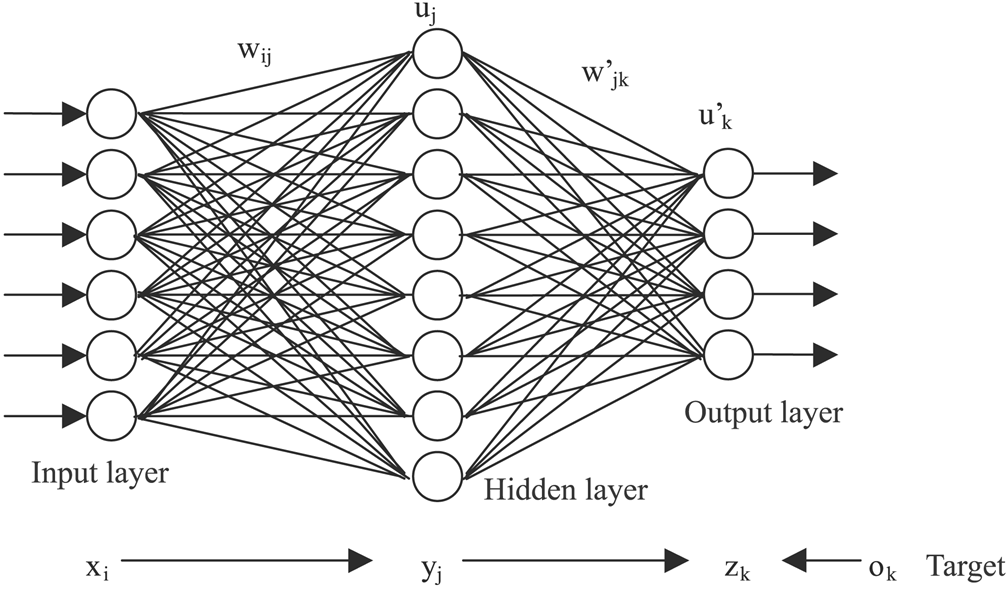
\includegraphics[width=0.5\textwidth]{ann.png}
\caption[width=0.5\textwidth]{Abstract representation of a feed-forward ANN}
\end{figure}

The first model of an artificial neuron was proposed by Walter Pitts and MuCulloch in 1943. This neuron computes a weighted sum of its inputs and generates an output of 1 if the sum is above a threshold, or 0 otherwise. 
\begin{figure}[h]
\centering
\label {fig: pitt}
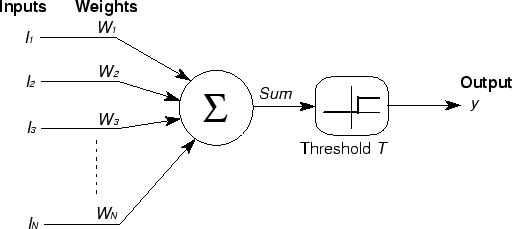
\includegraphics[width=0.5\textwidth]{pitts.png}
\caption[width=0.5\textwidth]{The MuCulloch-Pitts neuron}
\end{figure}

This kind of neuron has been further generalized. Instead of a threshold, an activation function is used, such as Gaussian, sigmoid and piecewise linear. We chose the rectifier as our activation function for its simplicity and its better gradient propagation:
$F(x) = x_{}^{+} = max(0, x)$

Based on the architecture, we can group ANNs into two: feed-forward networks, where the information flows in one direction, and recurrent networks, loops occur so we can better process sequential data. We will be using the latter to implement our algorithm.


\subsection {Recurrent Neural Network}

As mentioned before, Recurrent Neural Networks (RNNs) are a class of dynamic models, used when a sequence of data needs be processed and generated. They were first proposed in the 80’s for modelling time series. They compute a sequence one element at a time, while maintaining a “history” of all past elements. We could also view the structure of the network similar to that of a deep multilayer feed-forward network, with the outputs of the hidden units at previous steps as inputs of different neurons at the current step. This visualization makes it easy to see how backpropagation can be implemented in a regular RNN.
\begin{figure}[h]
\centering
\label {fig: rnn}
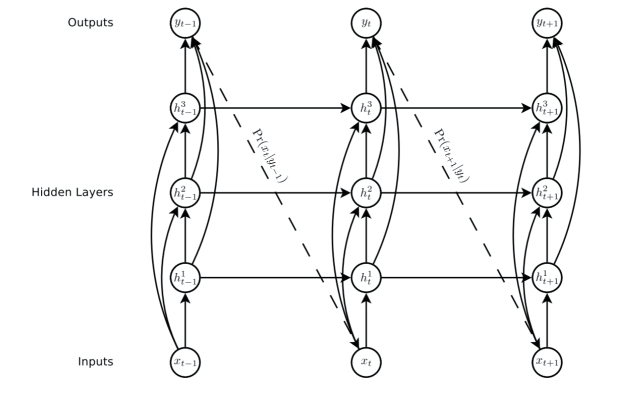
\includegraphics[width=0.5\textwidth]{rnn.png}
\caption[width=0.5\textwidth]{Deep RNN (prediction) architecture}
\end{figure}

Training RNNs proved to be a difficult task, as the backpropagated gradients tend to get either too big, or too small from a step to another, making some data be irrelevant or quite the opposite. These problems are referred to as the vanishing gradient and the exploding gradient, the first one being the more encountered of the two.

RNNs are being used to generate sequences in various domains such as music, text processing and even motion capture data. This dynamic model looks like a promising approach to our audio separation task, giving that we take care of the vanishing gradient.

\subsection {Vanishing gradient}

RNNs need to learn which past inputs have to be stored and how important they are to compute the current desired output. Because of this, backpropagation suffers from a too long learning time, as the time lag between inputs and relevant stored signals are extended. Error signals propagating back in time tend to vanish, making long-term dependencies hard to achieve or almost impossible to train. We will look over a few methods to prevent the problem of vanishing gradients.

Introducing time constants could help with long time lags, by modifying the unit activations. Related to this, a time-delay network called NARX networks were designed and proposed to take care of the vanishing gradient problem. The solution lies mostly in implementing “shortcuts” in the error backpropagation. This does not solve the root problem, but is an improvement to the regular design of a RNN.

A naive solution is searching without gradients. Instead of a continuous optimization that guides the weight search, various other search methods are used. The simplest example is by initializing randomly, until acceptable outputs to the available inputs are found. Weight guessing is not a good algorithm, but with certain optimizations it can lead to a realistic solution to certain easy tasks.  

Currently, the most efficient solution to the vanishing gradient, is “Long Short-Term Memory” (LSTM), a gradient based method that truncates the gradient when it doesn’t harm. Further, we will explain this method in detail, as it will be used in the architecture of our RNN. 


\subsection {Long Short-Term Memory}

Long Short-Term Memory has proved to be a more efficient, easier to train architecture than conventional RNNs. First theorized in 1997 by Hochreiter and Schmidhuber, it drew a lot of attention in the deep learning community, and obtained good results in tasks such as music composition or speech recognition. LSTM derives from the simple RNN architecture, the core of the first being the LSTM cell, a memory cell that is better at finding and exploiting long term dependencies. An LSTM cell is a structure made of different gates that control how the information flows to hidden neurons.


\begin{figure}[h]
\centering
\label {fig: lstmcell}
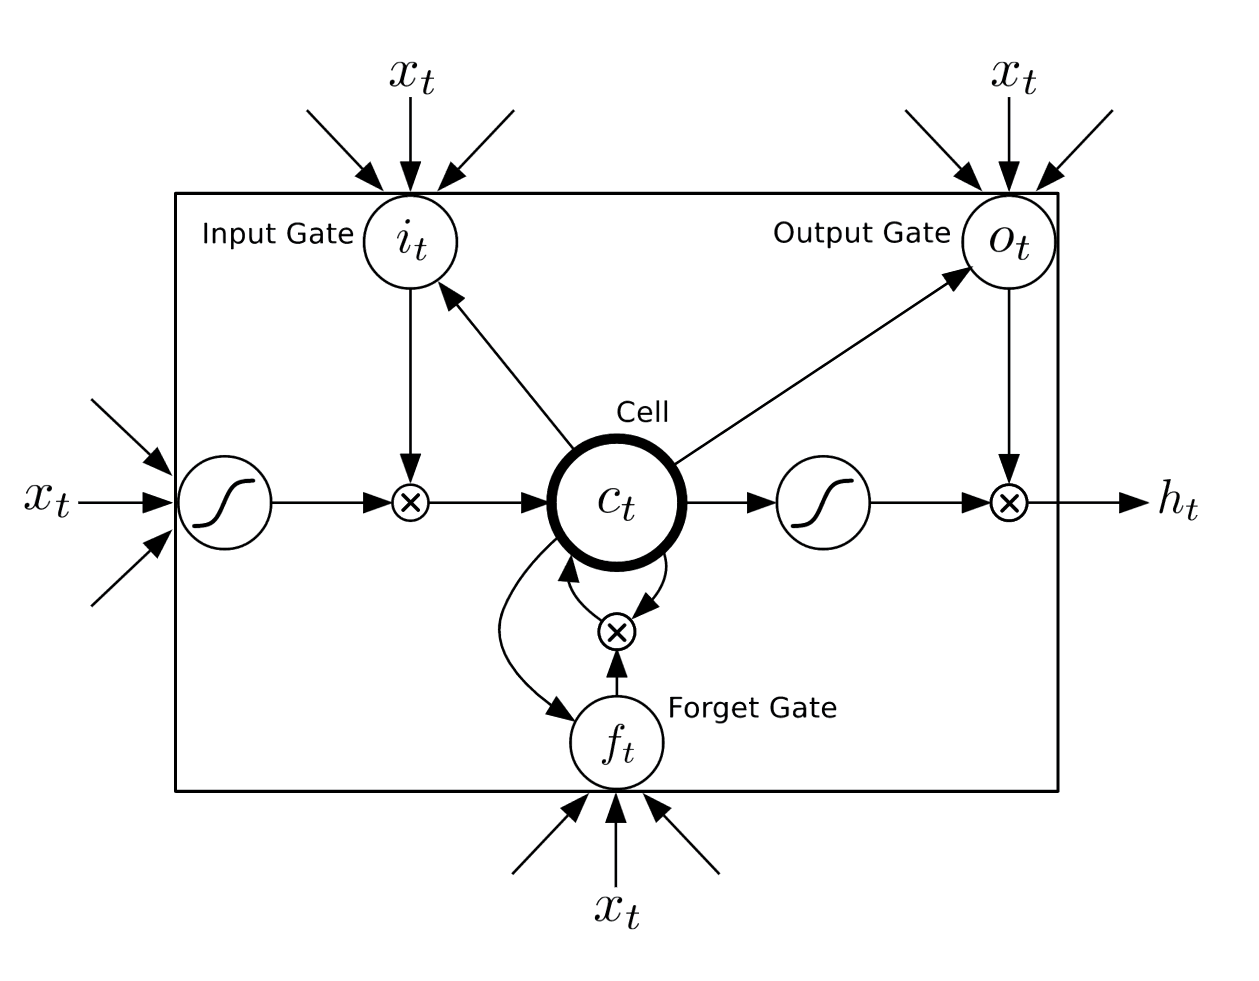
\includegraphics[width=0.5\textwidth]{lstmcell.png}
\caption[width=0.5\textwidth]{LSTM Cell}
\end{figure}

Figure 2.5 portrays a basic LSTM Cell, where $i$ is the input gate, $o$ is the output gate, $f$ is the forget gate and $c$ is the cell input activation vector. All these are the same size as the vector $h$. The below functions describe hoe information flows through these gates/actiavtion vectors.
\[ \mathit{i}_{\mathit{t}} = \sigma (W_{\mathit{xi}} \mathit{x}_\mathit{t} + W_{\mathit{hi}}  \mathit{h}_{\mathit{t} - 1} + W_{\mathit{ci}}  \mathit{c}_{\mathit{t} - 1} + \mathit{b}_\mathit{i}) \]
\[ \mathit{f}_{\mathit{t}} = \sigma (W_{\mathit{xf}} \mathit{x}_\mathit{t} + W_{\mathit{hf}}  \mathit{h}_{\mathit{t} - 1} + W_{\mathit{cf}}  \mathit{c}_{\mathit{t} - 1} + \mathit{b}_\mathit{f}) \]
\[ \mathit{f}_{\mathit{t}} = \mathit{f}_\mathit{t} \mathit{c}_{\mathit{t} - 1} +  \mathit{i}_\mathit{t} tanh (W_{\mathit{xc}} \mathit{x}_\mathit{t} + W_{\mathit{hc}}  \mathit{h}_{\mathit{t} - 1} + \mathit{b}_\mathit{c}) \]
\[ \mathit{f}_{\mathit{t}} = \sigma (W_{\mathit{xo}} \mathit{x}_\mathit{t} + W_{\mathit{ho}}  \mathit{h}_{\mathit{t} - 1} + W_{\mathit{co}}  \mathit{c}_\mathit{t} + \mathit{b}_\mathit{o}) \]
\[ \mathit{h}_\mathit{t} = \mathit{o}_\mathit{t} tanh( \mathit{c}_\mathit{t} ) \]
\subsection {Overfitting}

Overfitting is a problem that occurs in our model, when the performance of the network improves for the training data but the network keeps performing worse for “unseen”, evaluation data. This may happen from multiple reasons, but most frequently by including more variable parameters than necessary, or by simply not feeding the network with enough training data. Basic feedforward neural network regularizations do not work with RNNs.
 
We are going to talk about 2 techniques that will help reduce overfitting of our data. The more intuitive solution is to multiply our training data. This is actually possible through data augmentation. To augment our dataset, we need to find a way to modify our input while keeping the expected output the same. This helps the neural network to better find the important (relevant) features. Thinking back to our problem, one way to augment our data is to add some background noise to each song and keep the same output. The training dataset will double in size and overfitting will most certainly reduce.

In regular deep networks, dropout is the most common technique for reducing overfitting, where random network neurons are masked during training. Unfortunately, we cannot apply this to our LSTM RNN. A similar weight-dropping technique might work. This requires setting random set of weights to 0 from the hidden to hidden weight matrices. This solution would not impact the training speed and it should work on our chosen neural network architecture. A more technical review and experiments using this technique can be found in \cite{stephen} .


\subsection {Optimization}

The success of the Neural Network resides mostly in optimizing and fine-tuning the model for your specific task. Let’s further talk about some factors that influence our model’s performance.

First, just having a training dataset is not enough. The data must be correct and diverse so that the model can distinguish important features. A correlation between the quantity of data and the size of the neural network is also important to prevent overfitting and underfitting. To help the model find features in our data, we can use different preprocess techniques. In our case, instead of feeding the waveform into the network, we will first transform it using STFT and only give the magnitude spectra as input.

Second, fine tuning parameters is a process that takes a lot of time but is still as important. Things like learning rate, layer size or batch size have a huge impact on the output. For example, increasing the size of the training batch helps decrease the time for the gradient to converge. These parameters are usually tuned by successive experiments and evaluations. 

Last, we need to make sure we are using the optimal functions. Using a good loss function for computing our error and backpropagating it can help the learning curve significantly. Activation functions need to be chosen carefully according to our desired behavior for that specific layer. After the model is created, optimizing should be an ongoing process.


\end{document}
